
\input /home/asu/na/v/style/beamhead


\usetheme{default} 

\title[]{MathMagic}
\author[]{Arnab Chakraborty}
\institute{%
Indian Statistical Institute
}
\date{Oct 28, 2017}

\input{notesornot.spec}
\begin{document}
\large\bf




\begin{frame}\begin{textblock}{1}(0,0)0+2=2\end{textblock}\frametitle{{\color{red}\underline{\Large\bf
}}}\frametitle{\underline{\Large\bf
Get off the earth!}}
\begin{textblock}{10}(1,-2)\only<1>{
\begin{center}
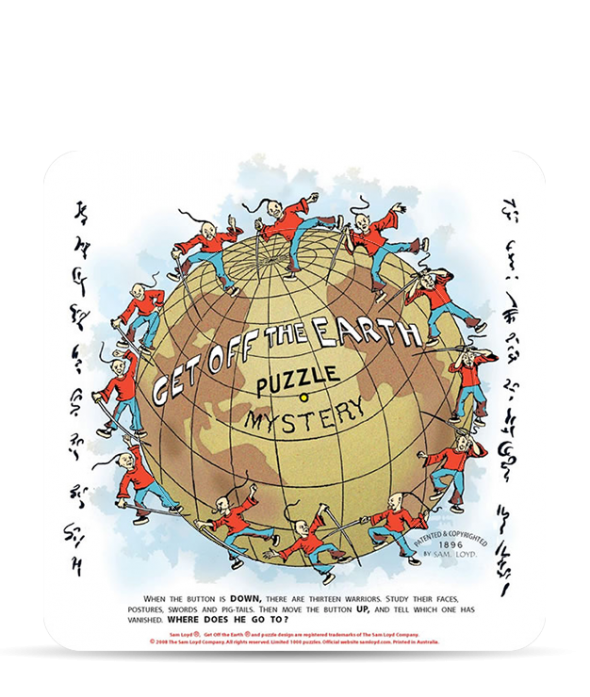
\includegraphics[scale=0.5]{image/goeclean1.png}\\
{\em \underline{How many men?}}
\end{center}
}%
\only<2>{
\begin{center}
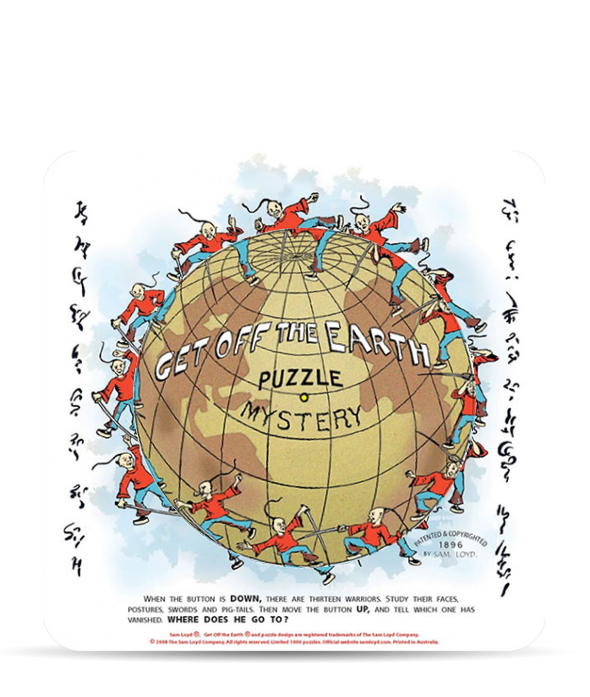
\includegraphics[scale=0.5]{image/goeclean2.png}\\
{\em \underline{How many men?}}
\end{center}
}%
\only<3>{
\begin{center}
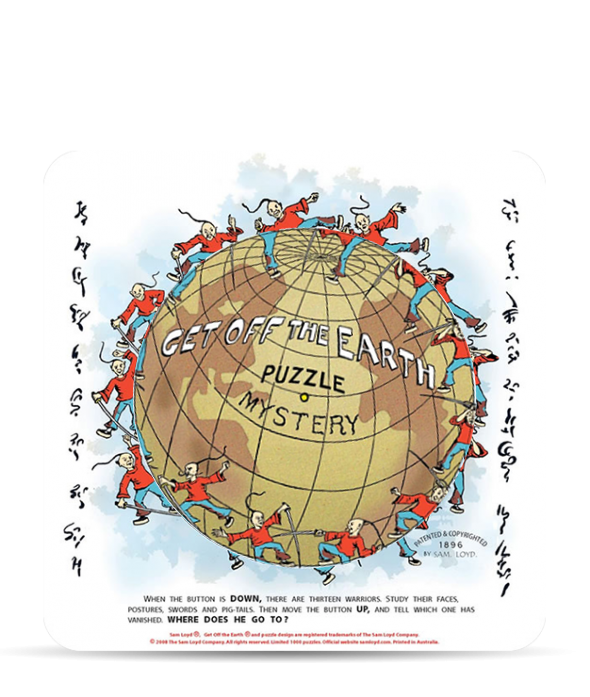
\includegraphics[scale=0.5]{image/goeclean3.png}\\
{\em \underline{How many men?}}
\end{center}
}%
\only<4>{
\begin{center}
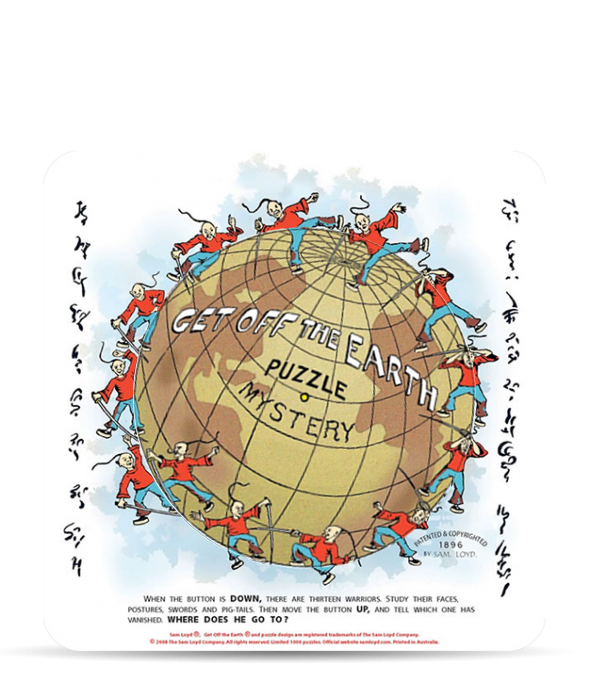
\includegraphics[scale=0.5]{image/goeclean4.png}\\
{\em \underline{How many men?}}
\end{center}
}%
\end{textblock}
\end{frame}

\begin{frame}\begin{textblock}{1}(0,0)2+2=4\end{textblock}\frametitle{{\color{red}\underline{\Large\bf
}}}\frametitle{\underline{\Large\bf
Mathematical perspective}}
\only<1>{
\begin{center}
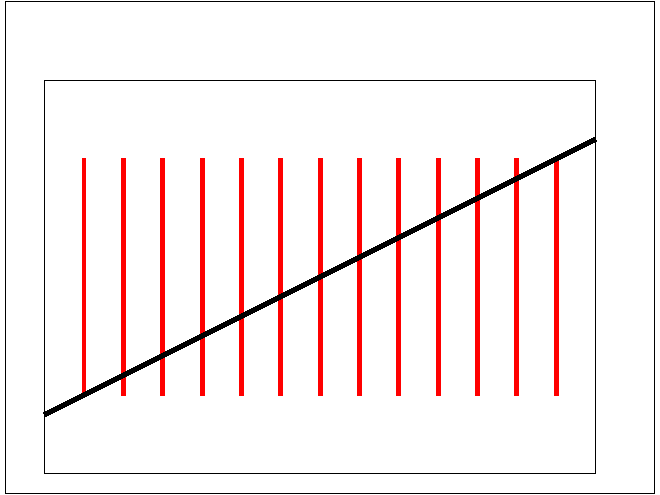
\includegraphics[scale=0.6]{image/linegoe1.pdf}\\
{\em \underline{}}
\end{center}
}%
\only<2>{
\begin{center}
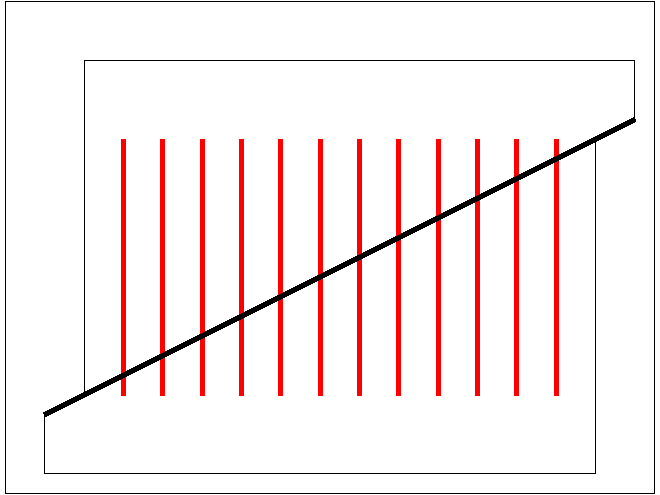
\includegraphics[scale=0.6]{image/linegoe2.pdf}\\
{\em \underline{}}
\end{center}
}%
\end{frame}

\begin{frame}\begin{textblock}{1}(0,0)4+2=6\end{textblock}\frametitle{{\color{red}\underline{\Large\bf
}}}\frametitle{\underline{\Large\bf
Making your own}}
\only<1>{
\begin{center}
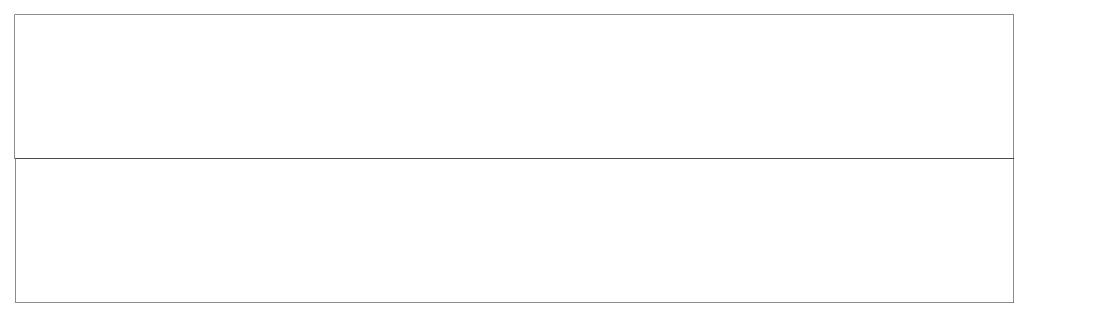
\includegraphics[scale=0.3]{image/fun0a.png}\\
{\em \underline{}}
\end{center}
}%
\only<2>{
\begin{center}
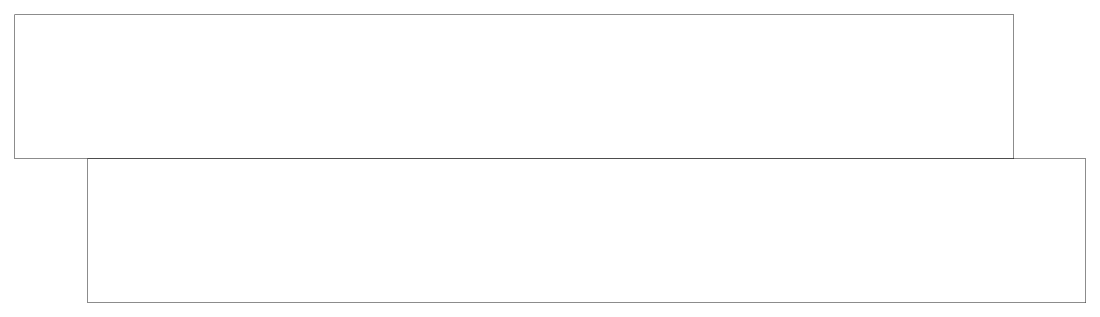
\includegraphics[scale=0.3]{image/fun0b.png}\\
{\em \underline{}}
\end{center}
}%
\only<3>{
\begin{center}
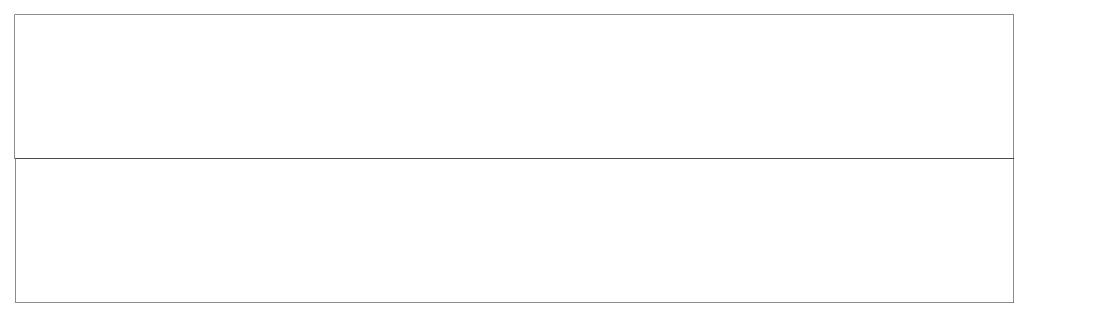
\includegraphics[scale=0.3]{image/fun0a.png}\\
{\em \underline{}}
\end{center}
}%
\only<4>{
\begin{center}
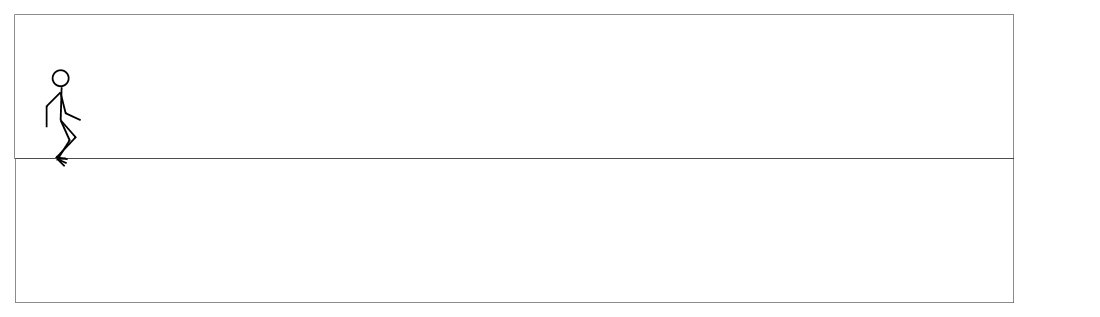
\includegraphics[scale=0.3]{image/fun1.png}\\
{\em \underline{}}
\end{center}
}%
\only<5>{
\begin{center}
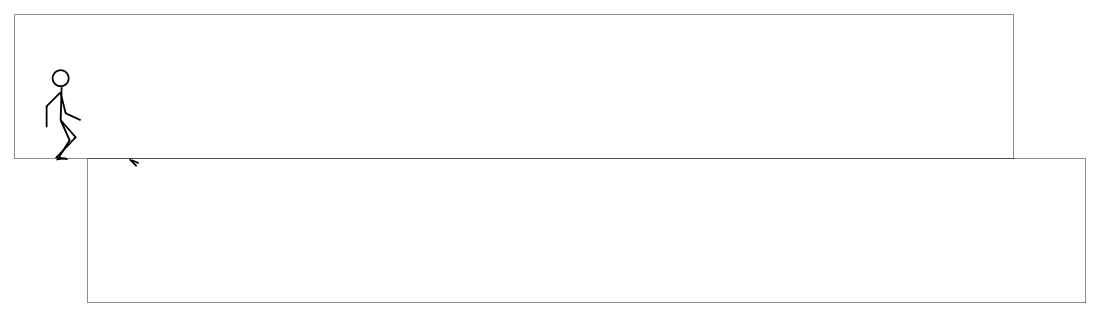
\includegraphics[scale=0.3]{image/fun2a.png}\\
{\em \underline{}}
\end{center}
}%
\only<6>{
\begin{center}
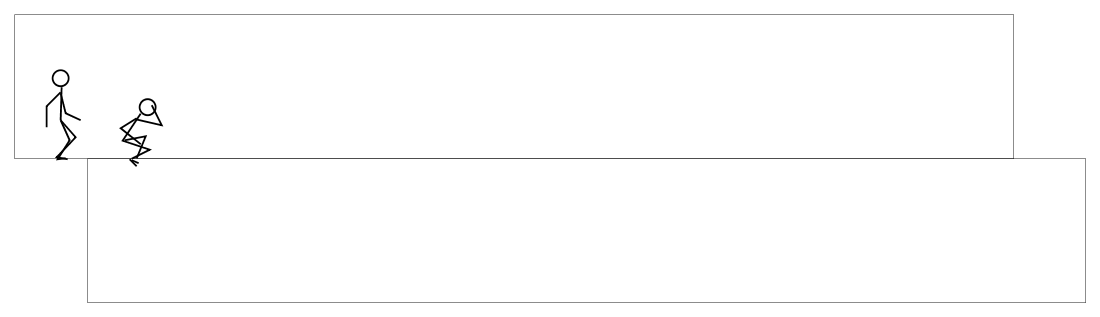
\includegraphics[scale=0.3]{image/fun2b.png}\\
{\em \underline{}}
\end{center}
}%
\only<7>{
\begin{center}
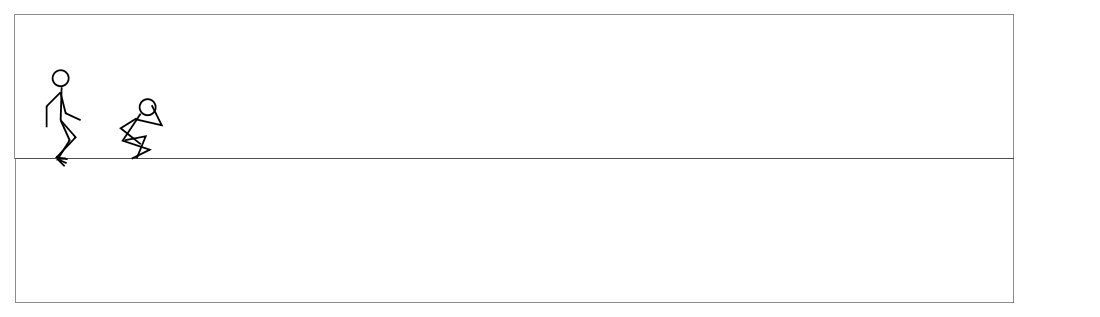
\includegraphics[scale=0.3]{image/fun3a.png}\\
{\em \underline{}}
\end{center}
}%
\only<8>{
\begin{center}
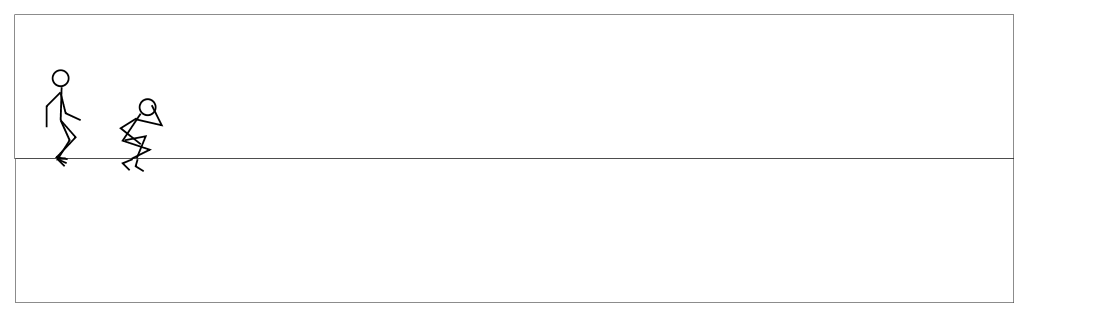
\includegraphics[scale=0.3]{image/fun3b.png}\\
{\em \underline{}}
\end{center}
}%
\only<9>{
\begin{center}
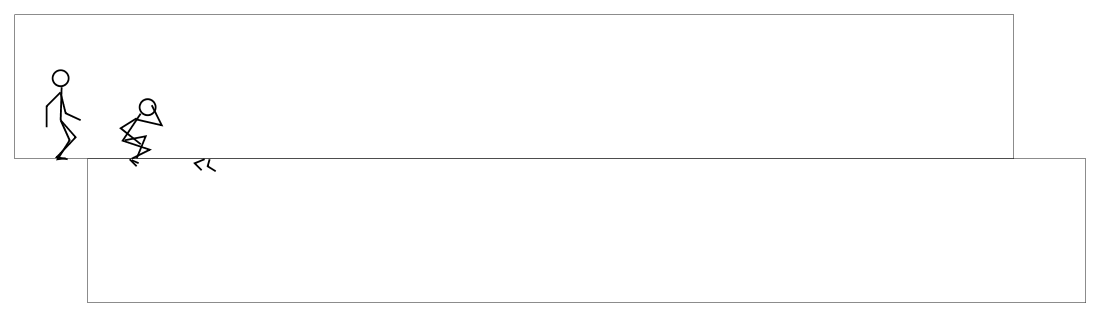
\includegraphics[scale=0.3]{image/fun4a.png}\\
{\em \underline{}}
\end{center}
}%
\only<10>{
\begin{center}
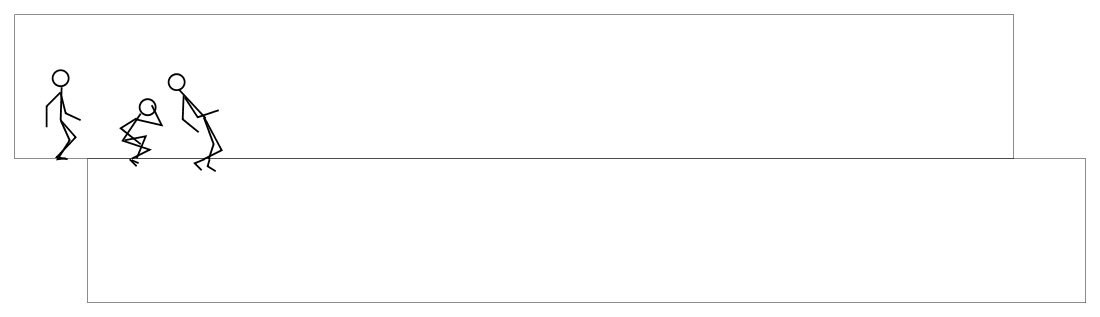
\includegraphics[scale=0.3]{image/fun4b.png}\\
{\em \underline{}}
\end{center}
}%
\only<11>{
\begin{center}
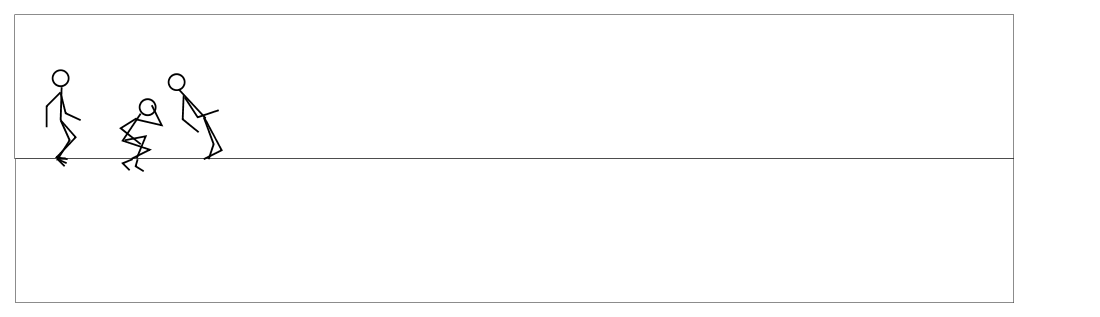
\includegraphics[scale=0.3]{image/fun5a.png}\\
{\em \underline{}}
\end{center}
}%
\only<12>{
\begin{center}
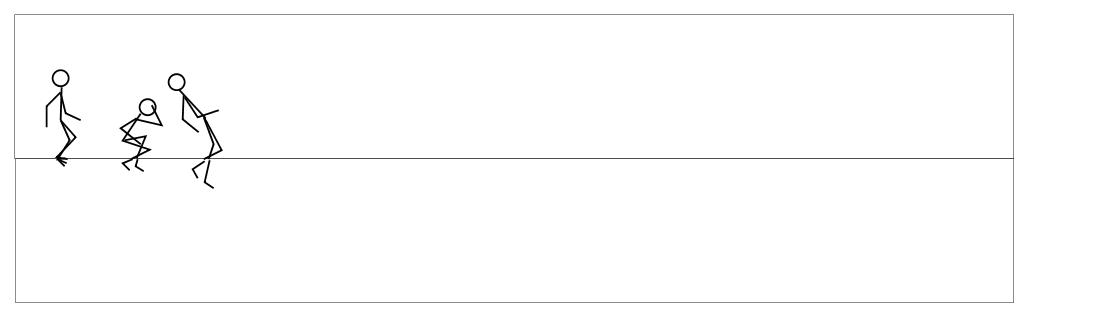
\includegraphics[scale=0.3]{image/fun5b.png}\\
{\em \underline{}}
\end{center}
}%
\only<13>{
\begin{center}
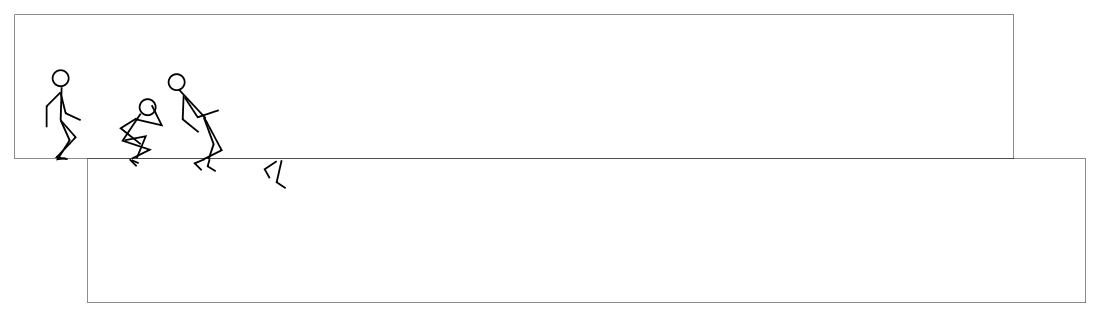
\includegraphics[scale=0.3]{image/fun6a.png}\\
{\em \underline{}}
\end{center}
}%
\only<14>{
\begin{center}
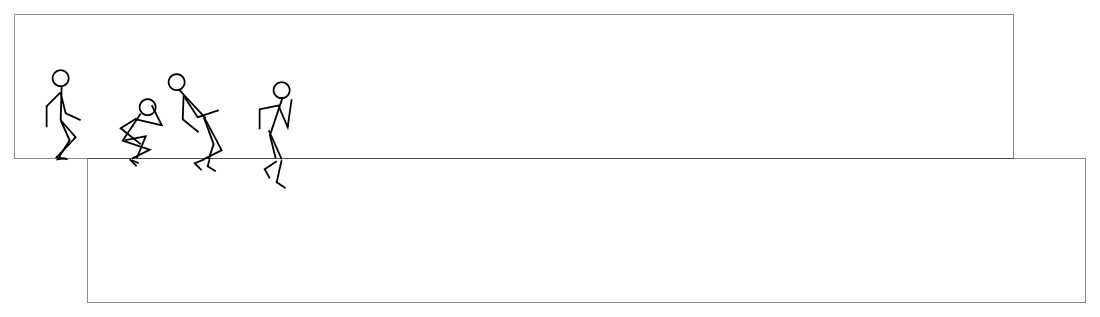
\includegraphics[scale=0.3]{image/fun6b.png}\\
{\em \underline{}}
\end{center}
}%
\only<15>{
\begin{center}
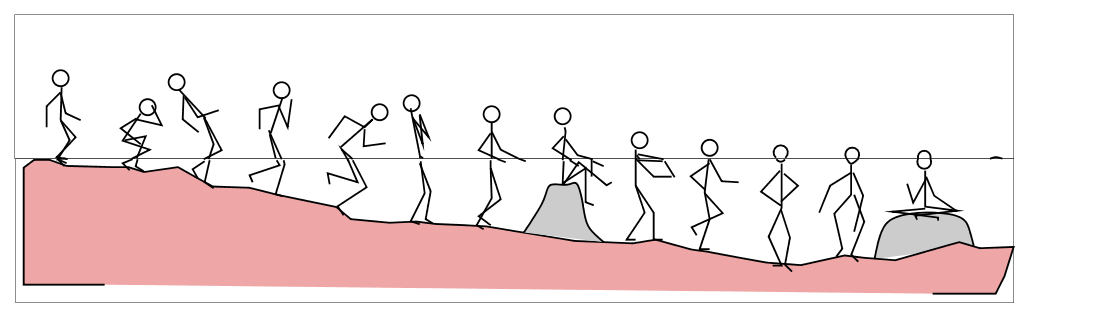
\includegraphics[scale=0.3]{image/funfulla.png}\\
{\em \underline{}}
\end{center}
}%
\only<16>{
\begin{center}
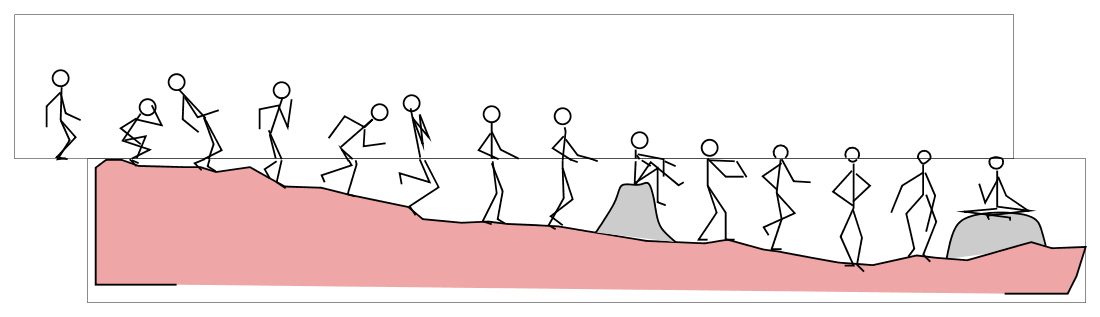
\includegraphics[scale=0.3]{image/funfullb.png}\\
{\em \underline{}}
\end{center}
}%
\end{frame}


\section{Puzzle}
\begin{frame}\begin{textblock}{1}(0,0)6+2=8\end{textblock}\frametitle{{\color{red}\underline{\Large\bf
}}}\frametitle{\underline{\Large\bf
Puzzle of the five cups}}

\centerline{\huge Invariance}
\end{frame}

\section{Magic}


\begin{frame}\begin{textblock}{1}(0,0)8+2=10\end{textblock}\frametitle{{\color{red}\underline{\Large\bf
}}}\frametitle{\underline{\Large\bf
Cut}}
\only<1>{
\begin{center}
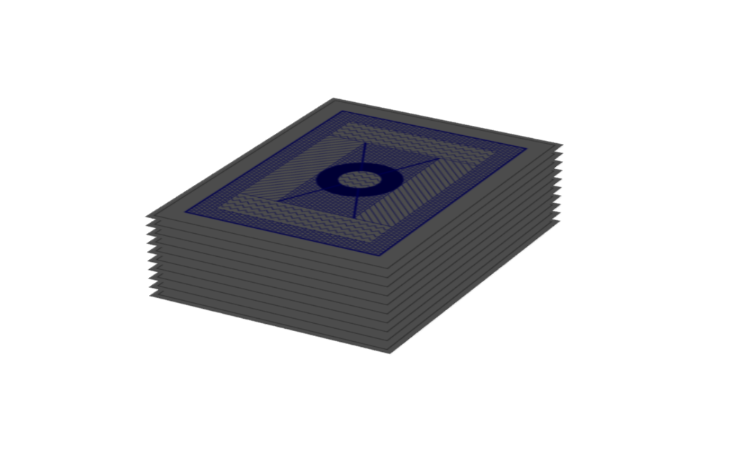
\includegraphics[scale=0.5]{image/hummer1.png}\\
{\em \underline{}}
\end{center}
}%
\only<2>{
\begin{center}
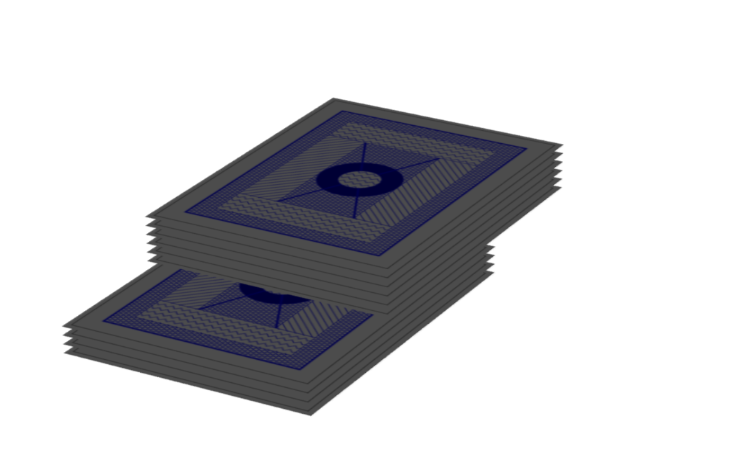
\includegraphics[scale=0.5]{image/hummer2.png}\\
{\em \underline{}}
\end{center}
}%
\only<3>{
\begin{center}
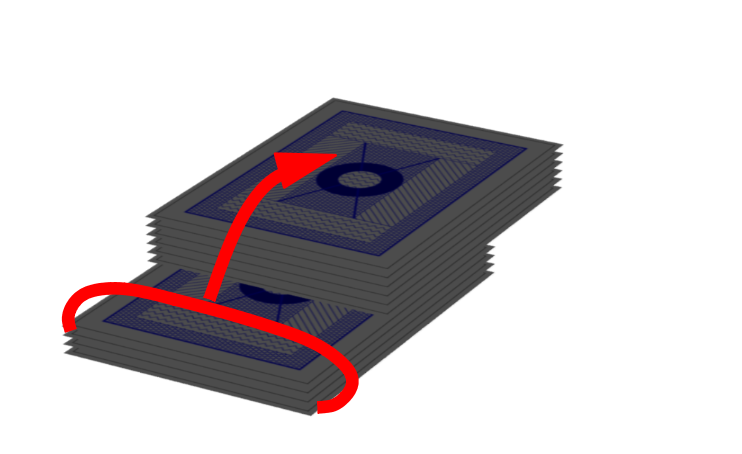
\includegraphics[scale=0.5]{image/hummer3.png}\\
{\em \underline{}}
\end{center}
}%
\end{frame}
\begin{frame}\begin{textblock}{1}(0,0)10+2=12\end{textblock}\frametitle{{\color{red}\underline{\Large\bf
}}}\frametitle{\underline{\Large\bf
Flip top two together}}
\only<1>{
\begin{center}
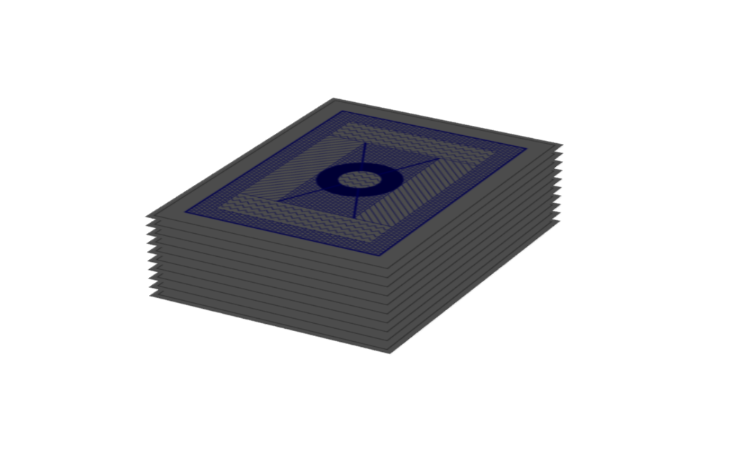
\includegraphics[scale=0.5]{image/hummer1.png}\\
{\em \underline{}}
\end{center}
}%
\only<2>{
\begin{center}
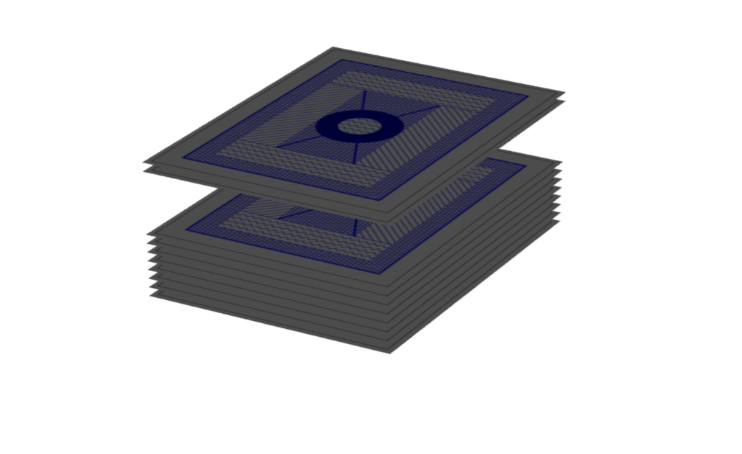
\includegraphics[scale=0.5]{image/hummer4.png}\\
{\em \underline{}}
\end{center}
}%
\only<3>{
\begin{center}
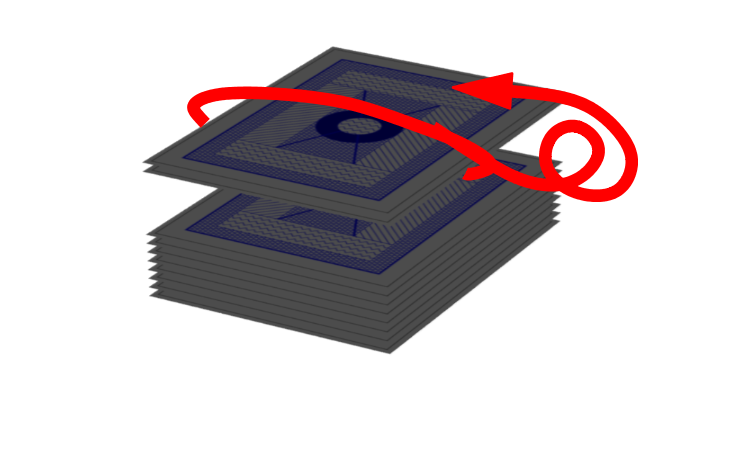
\includegraphics[scale=0.5]{image/hummer5.png}\\
{\em \underline{}}
\end{center}
}%
\end{frame}

\begin{frame}\begin{textblock}{1}(0,0)12+2=14\end{textblock}\frametitle{{\color{red}\underline{\Large\bf
}}}\frametitle{\underline{\Large\bf
Instructions}}

\begin{itemize}

\item Give a  random cut.
\item Remember the bottom card.
\item Take the top card to the bottom.
\item Flip the top card.
\item Random cut.
\item Flip top two cards together.
\item Repeat the above two steps $3$ times.
\item Give me the packet.

\end{itemize}

\end{frame}

\section{Euler}

\begin{frame}\begin{textblock}{1}(0,0)14+2=16\end{textblock}\frametitle{{\color{red}\underline{\Large\bf
}}}\frametitle{\underline{\Large\bf
From high school days}}
\only<1>{
\begin{center}
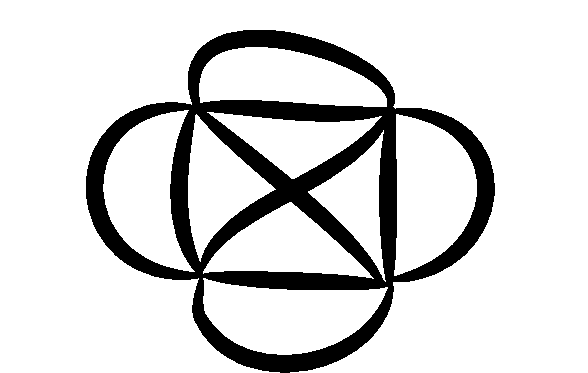
\includegraphics[scale=0.5]{image/euler1.pdf}\\
{\em \underline{}}
\end{center}
}%
\only<2>{
\begin{center}
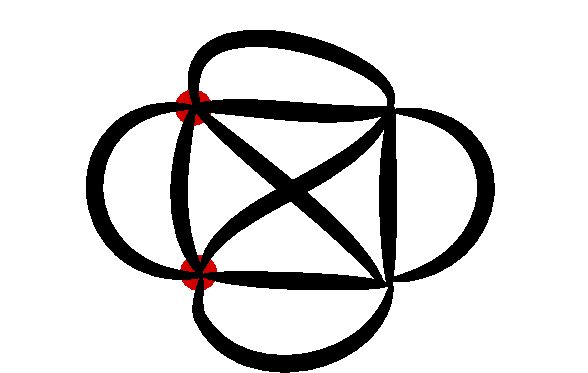
\includegraphics[scale=0.5]{image/euler2.pdf}\\
{\em \underline{}}
\end{center}
}%
\only<3>{
\begin{center}
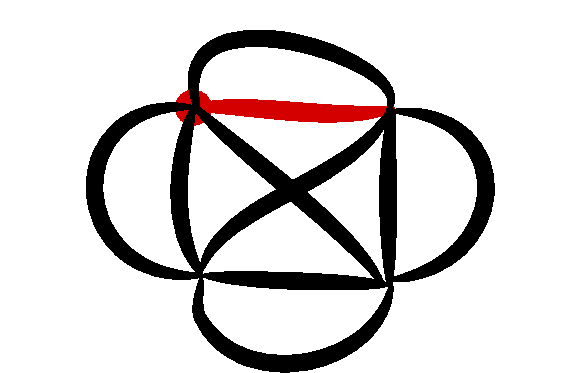
\includegraphics[scale=0.5]{image/euler3.pdf}\\
{\em \underline{}}
\end{center}
}%
\only<4>{
\begin{center}
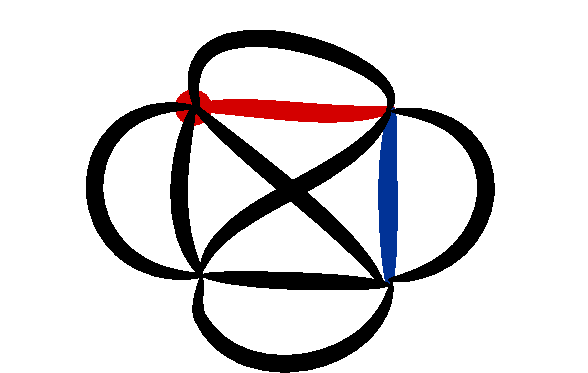
\includegraphics[scale=0.5]{image/euler4.pdf}\\
{\em \underline{}}
\end{center}
}%
\end{frame}
\begin{frame}\begin{textblock}{1}(0,0)16+2=18\end{textblock}\frametitle{{\color{red}\underline{\Large\bf
}}}\frametitle{\underline{\Large\bf
Euler's theorem}}
Consider a diagram consisting of some points
joined by some lines such that you can go from any point to any
other point. Then you can draw this diagram without lifting your
pen and without  reusing any line if and only if 

\begin{quote}
either 
  
\begin{quote}
only an even number of lines meet at each point
\end{quote}

or

\begin{quote}
an odd number of lines meet at exactly two points
\end{quote}
  

\end{quote}

\end{frame}
\begin{frame}\begin{textblock}{1}(0,0)18+2=20\end{textblock}\frametitle{{\color{red}\underline{\Large\bf
}}}\frametitle{\underline{\Large\bf
An example}}

\only<1>{\begin{center}
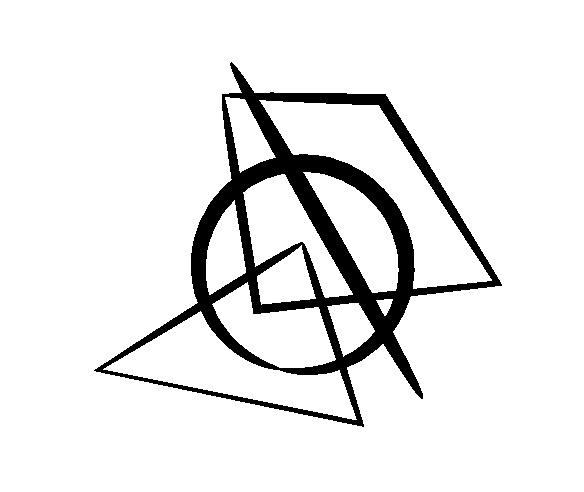
\includegraphics[scale=0.5]{image/eul1.pdf}\\
{\em \underline{}}
\end{center}}%
\only<2->{\begin{center}
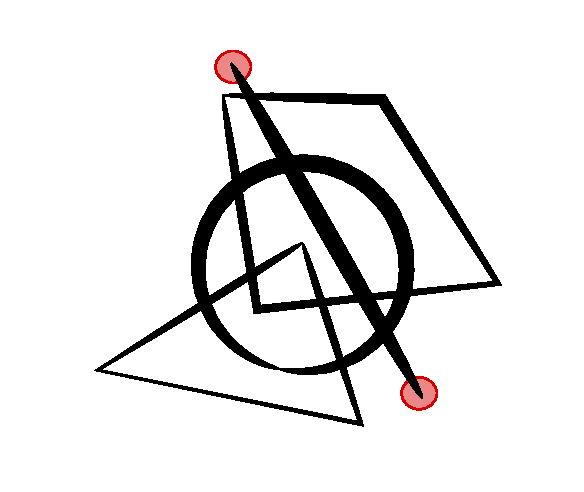
\includegraphics[scale=0.5]{image/eul2.pdf}\\
{\em \underline{}}
\end{center}}%
\end{frame}

\begin{frame}\begin{textblock}{1}(0,0)20+2=22\end{textblock}\frametitle{{\color{red}\underline{\Large\bf
}}}\frametitle{\underline{\Large\bf
Mind reading magic}}
\end{frame}
\subsection{Explanation}
\begin{frame}\begin{textblock}{1}(0,0)22+2=24\end{textblock}\frametitle{{\color{red}\underline{\Large\bf
}}}\frametitle{\underline{\Large\bf
Did I do it without {\color{red}any} information?}}

\only<1>{
\begin{center}
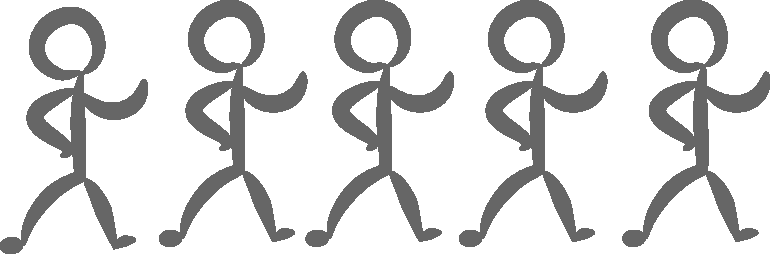
\includegraphics[scale=0.5]{image/people1.pdf}\\
{\em \underline{}}
\end{center}
}%
\only<2->{
\begin{center}
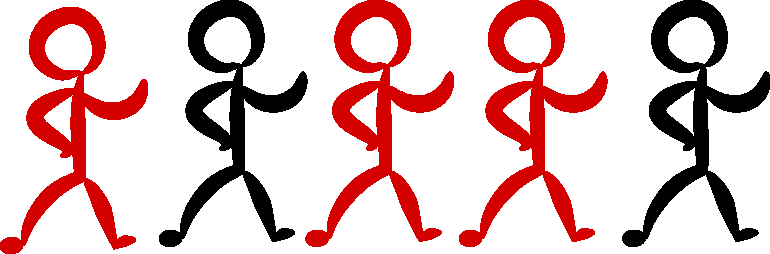
\includegraphics[scale=0.5]{image/people2.pdf}\\
{\em \underline{}}
\end{center}
}%

\uncover<3->{How many such patterns are possible?}


\vspace{1cm }


\uncover<4>{Ans: $2^5.$}
\end{frame}

\begin{frame}\begin{textblock}{1}(0,0)24+2=26\end{textblock}\frametitle{{\color{red}\underline{\Large\bf
}}}\frametitle{\underline{\Large\bf
A deck of (at most) 32 cards}}
\uncover<2->{Hmmm...so you used an arranged deck!}% 


\vspace{1cm }


\uncover<3->{But did we not shuffle it thoroughly?}%
\begin{textblock}{10}(1,6)\only<4>{
\begin{center}
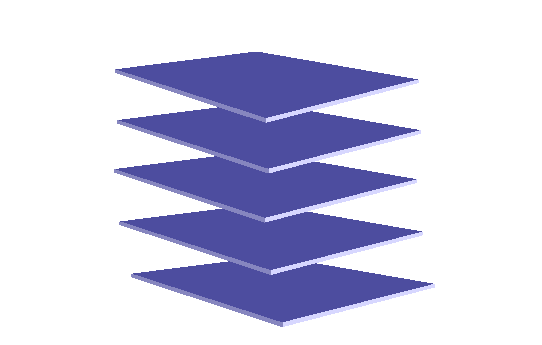
\includegraphics[scale=0.5]{image/deckcycle1.pdf}\\
{\em \underline{}}
\end{center}
}%
\only<5>{
\begin{center}
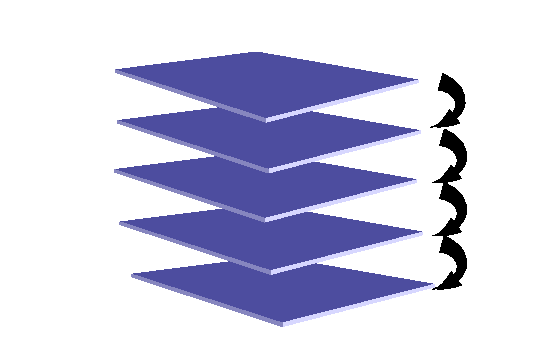
\includegraphics[scale=0.5]{image/deckcycle2.pdf}\\
{\em \underline{}}
\end{center}
}%
\only<6->{
\begin{center}
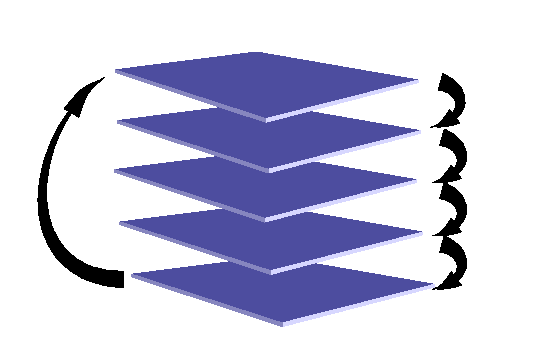
\includegraphics[scale=0.5]{image/deckcycle3.pdf}\\
{\em \underline{}}
\end{center}
}%
\end{textblock}
\begin{textblock}{10}(5,6)\only<4-6>{
\begin{center}
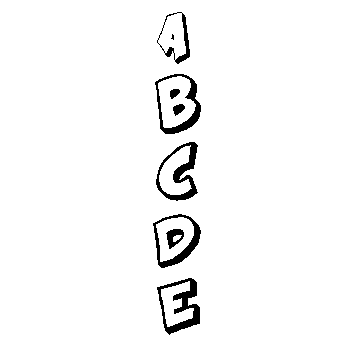
\includegraphics[scale=0.5]{image/cy1.pdf}\\
{\em \underline{}}
\end{center}
}%
\only<7>{
\begin{center}
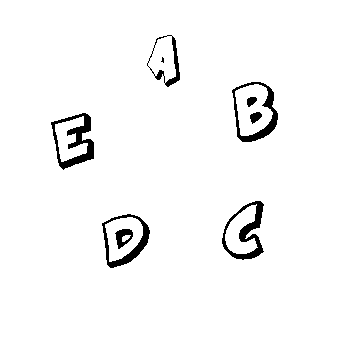
\includegraphics[scale=0.5]{image/cy2.pdf}\\
{\em \underline{}}
\end{center}
}%
\end{textblock}
\end{frame}

\begin{frame}\begin{textblock}{1}(0,0)26+2=28\end{textblock}\frametitle{{\color{red}\underline{\Large\bf
}}}\frametitle{\underline{\Large\bf
OK, cyclical arrangement. But how?}}
\begin{textblock}{10}(2,2)
\only<2>{
\begin{center}
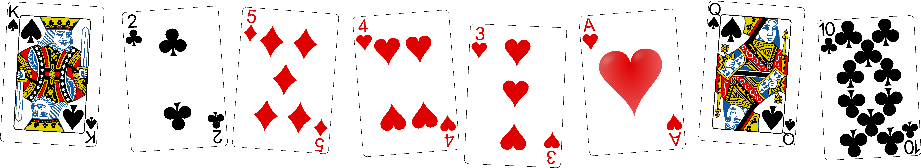
\includegraphics[scale=0.5]{image/8cards1.pdf}\\
{\em \underline{$2^3=8$ cards}}
\end{center}
}%
\only<3>{
\begin{center}
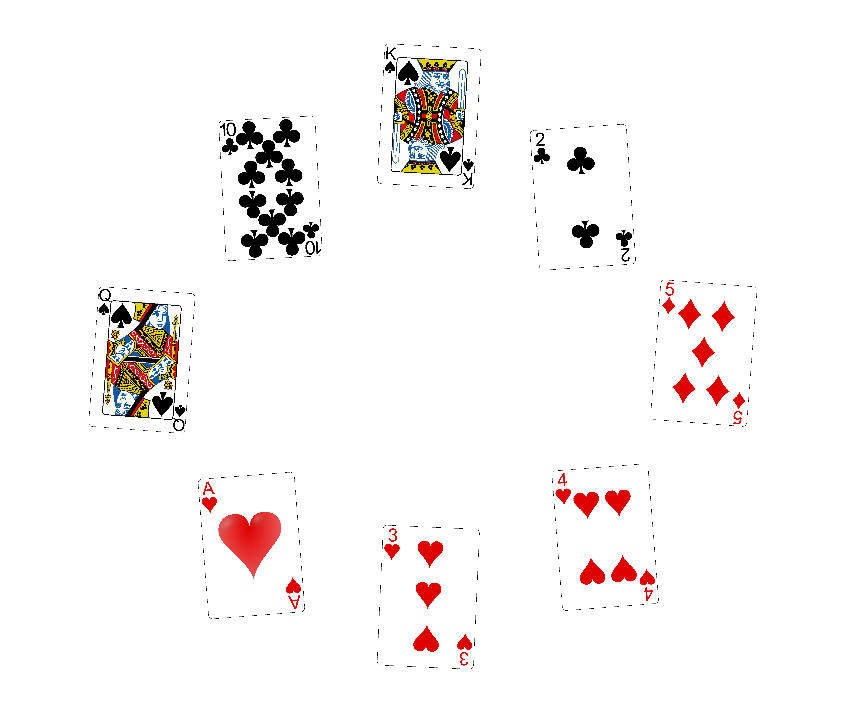
\includegraphics[scale=0.5]{image/8cards2.pdf}\\
{\em \underline{Is this arrangement OK?}}
\end{center}
}%
\only<4>{
\begin{center}
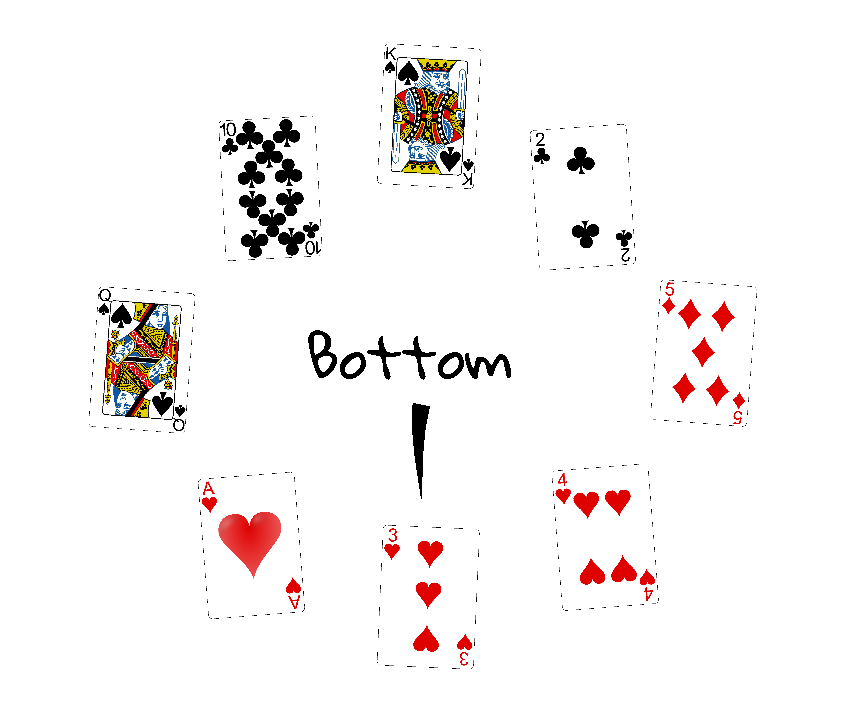
\includegraphics[scale=0.5]{image/8cards3a.pdf}\\
{\em \underline{Is this arrangement OK?}}
\end{center}
}%
\only<5>{
\begin{center}
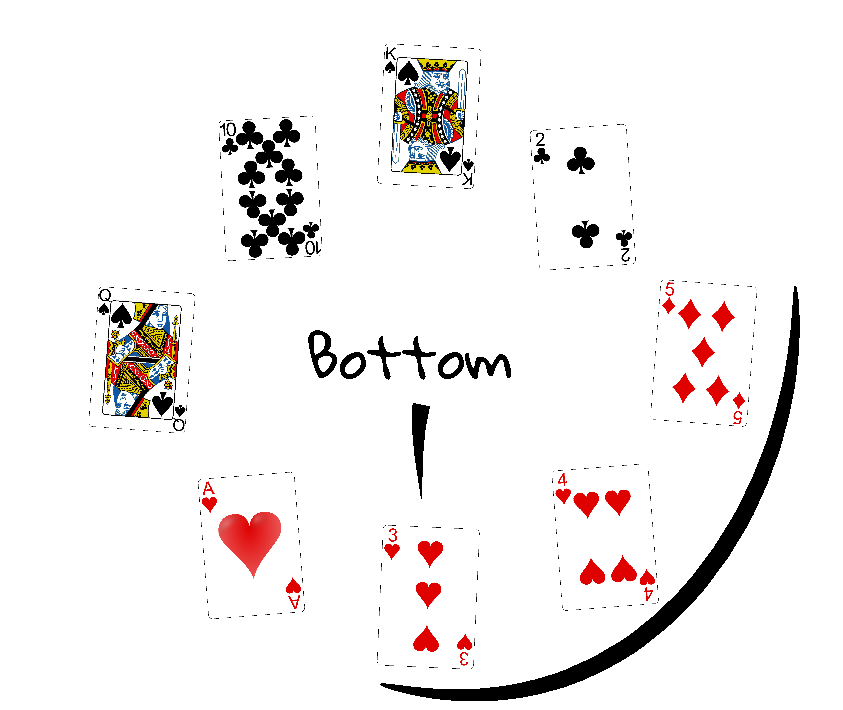
\includegraphics[scale=0.5]{image/8cards3b.pdf}\\
{\em \underline{Is this arrangement OK?}}
\end{center}
}%
\only<6>{
\begin{center}
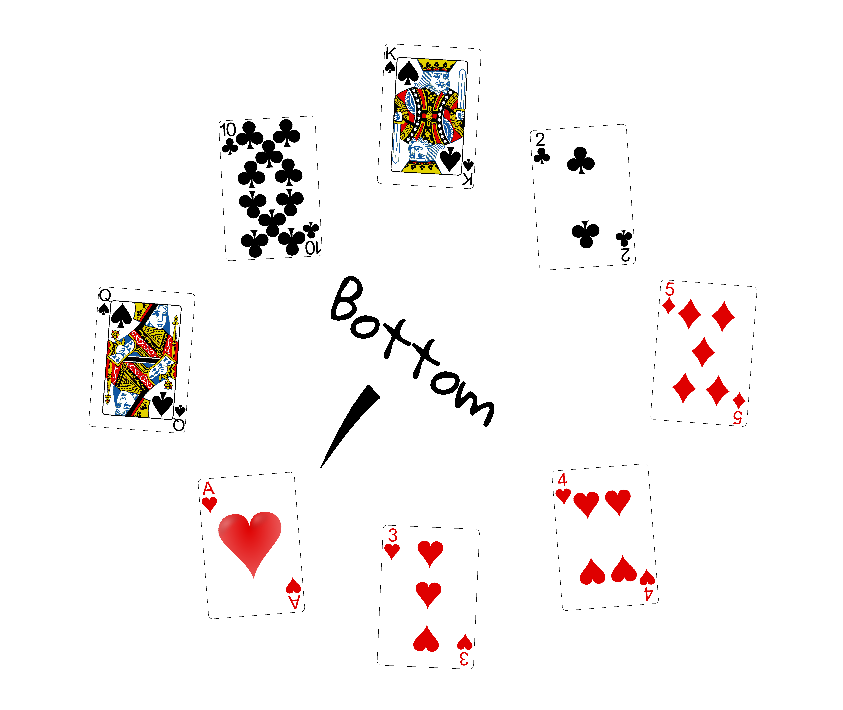
\includegraphics[scale=0.5]{image/8cards4a.pdf}\\
{\em \underline{Is this arrangement OK?}}
\end{center}
}%
\only<7>{
\begin{center}
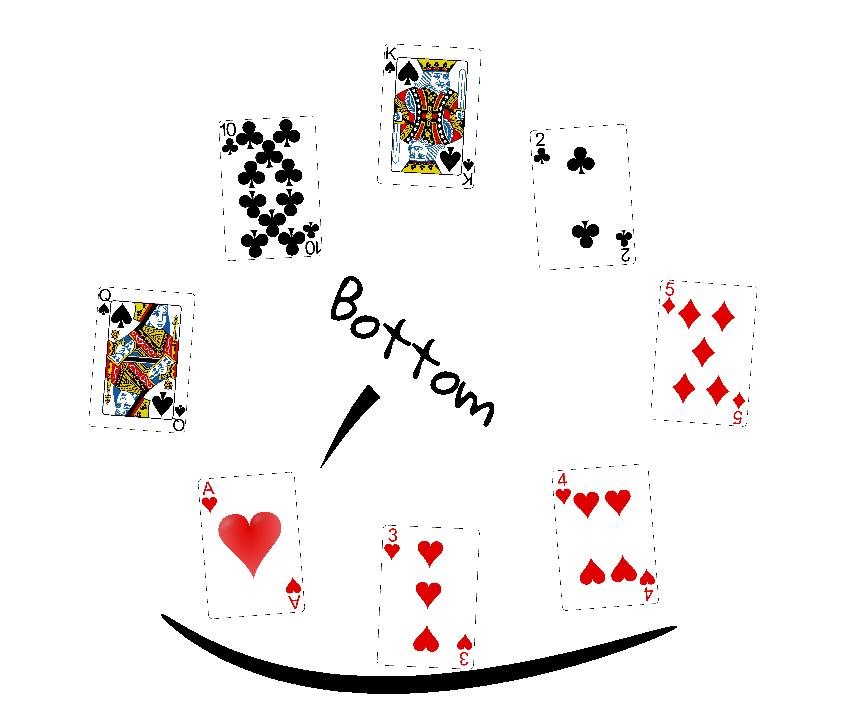
\includegraphics[scale=0.5]{image/8cards4b.pdf}\\
{\em \underline{Is this arrangement OK?}}
\end{center}
}%
\end{textblock}
\begin{textblock}{10}(6,2)
\only<4,6>{
\begin{center}
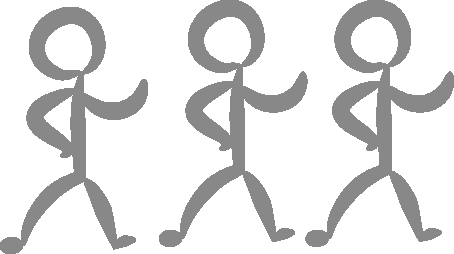
\includegraphics[scale=0.3]{image/tinjan1.pdf}\\
{\em \underline{}}
\end{center}
}%
\only<5,7>{
\begin{center}
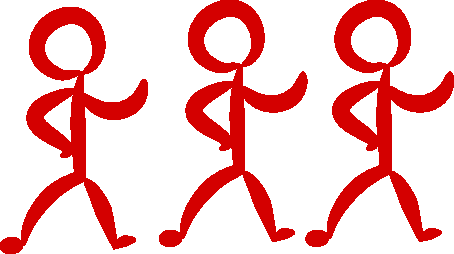
\includegraphics[scale=0.3]{image/tinjan2.pdf}\\
{\em \underline{}}
\end{center}
}%
\end{textblock}
\end{frame}

\begin{frame}\begin{textblock}{1}(0,0)28+2=30\end{textblock}\frametitle{{\color{red}\underline{\Large\bf
}}}\frametitle{\underline{\Large\bf
So we need...}}
...a cyclical pattern where all consecutive triples have distinct
red-black patterns.
\only<1>{
\begin{center}
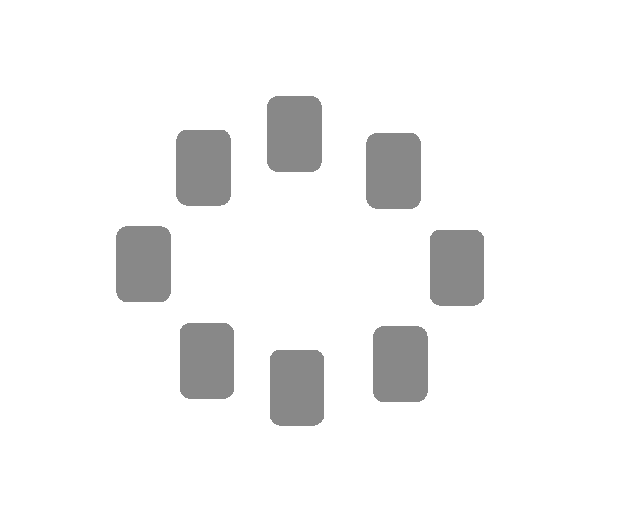
\includegraphics[scale=0.5]{image/allpat0.pdf}\\
{\em \underline{}}
\end{center}
}%
\only<2>{
\begin{center}
\includegraphics[scale=0.5]{image/allpat1.pdf}\\
{\em \underline{}}
\end{center}
}%
\only<3>{
\begin{center}
\includegraphics[scale=0.5]{image/allpat2.pdf}\\
{\em \underline{}}
\end{center}
}%
\only<4>{
\begin{center}
\includegraphics[scale=0.5]{image/allpat3.pdf}\\
{\em \underline{}}
\end{center}
}%
\only<5>{
\begin{center}
\includegraphics[scale=0.5]{image/allpat4.pdf}\\
{\em \underline{}}
\end{center}
}%
\only<6>{
\begin{center}
\includegraphics[scale=0.5]{image/allpat5.pdf}\\
{\em \underline{}}
\end{center}
}%
\only<7>{
\begin{center}
\includegraphics[scale=0.5]{image/allpat6.pdf}\\
{\em \underline{}}
\end{center}
}%
\only<8>{
\begin{center}
\includegraphics[scale=0.5]{image/allpat7.pdf}\\
{\em \underline{}}
\end{center}
}%
\only<9->{
\begin{center}
\includegraphics[scale=0.5]{image/allpat8.pdf}\\
{\em \underline{}}
\end{center}
}%
\uncover<9->{How to find such a pattern?}

\uncover<10>{Does one really exist at all?}
\end{frame}






\end{document}
